% !TEX root = paper.tex
\section{Background and Motivation}
\label{sec:motivation}

\subsection{DOALL parallelization}

In DOALL parallelization, loop iterations need to run independently of each
other.
%
There cannot be any loop-carried (cross-iteration) memory flows (RAW
dependences), unless a reduction is identified. Loop-carried output and anti
(WAW and WAR) memory dependences need to be handled by privatization or
reduction. At the end of parallel invocation, workers need to merge their memory
states to a single live-out memory state.  Merging reduction objects is
inexpensive and does not require bookkeeping during the parallel invocation.
Merging private objects though can be very expensive. For every memory location
of private objects the last written value needs to be determined. If it cannot
be determined statically, then it needs to be tracked dynamically, resulting in
significant bookkeeping for all the involved stores.

\subsection{Automatic DOALL Software-only Systems}

\begin{table*}
  % !TEX root = ../paper.tex
\newcommand{\sbcheck}{\textcolor{ForestGreen}{\ding{51}}}
\newcommand{\sbcross}{\textcolor{RubineRed}{\ding{55}}}
\small
\centering
\begin{tabular}{|l|c|c|c|c|c|c|c|c|c|}
\hline
\multirow{2}{*}{Technique}   &
% \multirow{2}{*}{\parbox[c]{1.1cm}{\centering Fully\\ Automatic}} &
\multirow{2}{*}{\parbox[c]{1cm}{\centering Supports \\Spec}} &
\multirow{2}{*}{\parbox[c]{1.8cm}{\centering Supports Ptrs \\ and DynAlloc}} &
\multicolumn{2}{c|}{Supports Privatization} &
\multicolumn{2}{c|}{Supports Reduction} &
\multirow{2}{*}{\parbox[c]{1.4cm}{\centering Efficient \\Privatization}} &
\multirow{2}{*}{\parbox[c]{0.6cm}{\centering Cheap \\ Spec}} &
\multirow{2}{*}{\parbox[c]{1.7cm}{\centering \# Cores \\ Evaluated on}} \\

\cline{4-7}
&  &
& \parbox[c]{1cm}{\centering Static}   & \parbox[c]{1cm}{\centering Spec}
& \parbox[c]{1cm}{\centering Static} & \parbox[c]{1cm}{\centering Spec}
& & & \\ \hline

%%% LRPD %%%
\parbox[l]{2.4cm}{LRPD \cite{rauchwerger:95:sigplan,dang:02:ipdps}} & \sbcheck  & \sbcross & ?  & \sbcheck    & ?  & \sbcheck   & \sbcross    & \sbcross    & 14    \\ \hline

%%% Polaris %%%
\parbox[l]{2.4cm}{Polaris \cite{tu:94:lcpc,blume:96:icpp}} & \sbcross & \sbcross & \sbcheck    & \sbcross   & \sbcheck   & \sbcross  & \sbcheck    & \sbcross    & 8  \\ \hline

%%% SUIF %%%
\parbox[l]{2.4cm}{SUIF \cite{suif:94:stanford,hall:05:toplas}} & \sbcross & \sbcross & \sbcheck   & \sbcross   & \sbcheck  & \sbcross  & \sbcross    & \sbcross    & 4, 8   \\ \hline


%%% Sensitivity %%%
\parbox[l]{2.4cm}{Sensitivity \cite{Rus:07:ics}}  & \sbcheck  & \sbcross & \sbcheck    & \sbcheck    & \sbcheck   & \sbcheck   & \sbcheck     & ?    & 4 \\ \hline


%%% STMLite %%%
\parbox[l]{2.4cm} {STMLite \cite{mehrara:09:stmlite}} & \sbcheck  & \sbcheck  & \sbcheck   & \sbcheck   & \sbcross  & \sbcross  & \sbcross    & \sbcross    & 8 \\ \hline

% %%% Array Privatization %%%
% \parbox[l]{1.9cm}{Array \\Privatization\\ (Tu \& Padua)} & \sbcheck  & \sbcross & \sbcross & \sbcheck    & \sbcross   & \sbcross  & \sbcross  & \sbcheck     & \sbcross    & 8?    \\ \hline

%%% ClusterDOALL %%%
\parbox[l]{2.4cm}{ClusterDOALL \cite{kim:12:cgo}}  & \sbcheck  & \sbcheck  & \sbcross   & \sbcheck    & \sbcross  & \sbcross  & \sbcross & \sbcheck     & 120   \\ \hline

%%% Privateer %%%
\parbox[l]{2.4cm}{Privateer \cite{johnson:12:pldi}}  & \sbcheck  & \sbcheck  & \sbcross   & \sbcheck    & \sbcross  & \sbcheck   & \sbcross & \sbcheck     & 24    \\ \hline

%%% LSD %%%
\parbox[l]{2.4cm}{LSD (This work)} & \sbcheck  & \sbcheck  & \sbcheck    & \sbcheck    & \sbcheck   & \sbcheck   & \sbcheck     & \sbcheck     & 28    \\ \hline
\end{tabular}
  \caption{
    Comparison of LSD with Automatic DOALL software-only systems.
  }
  \label{tab:related-work}
    \vspace{-5pt}
\end{table*}

%To make a DOALL automatic on software-only systems, the most important job is to
%remove all loop-carried memory dependences. There are two ways to do it - the
%analysis-based or the speculation-based approach.

\subsubsection{Analysis-based Approaches}

With analysis, we can prove a dependence is not there or can be handled by
privatization or reduction, two major enablers for parallelism. Early works
%including SUIF~\cite{blume:96:icpp} and Polaris~\cite{suif:94:stanford}
% TODO: cite one static analysis only work here
used only static analysis to remove dependences. Using static analysis means all
the information should be available at compile time. However, there are a lot of
programs with input-sensitive dependences which are removable for certain
inputs. A line of work based on Polaris, namely LD~\cite{rauchwerger:94:ics},
LRPD~\cite{rauchwerger:99:pds}, and R-LRPD~\cite{dang:02:ipdps}, leverages
run-time analysis to check dependences based on the input and extends the
applicability of analysis-based DOALL systems.  Hybrid
Analysis~\cite{rus:03:hybrid} and Sensitivity Analysis~\cite{Rus:07:ics} combine
static analysis and run-time analysis to generate cheap predicates for memory
dependences, which reduce the run-time overhead.

Analysis-based systems when applicable can deliver good predictable
speedups~\cite{campanoni:2012:iscgo, raman:2008:iscgo, suif:94:stanford,
Rus:07:ics}, especially for scientific benchmarks.
% However, with the wide adoption of
% programming languages, with dynamic memory allocation and pointers, e.g., C and
% C++.
% TODO: change word "obvious"
However, the shortcomings of analysis-based systems are obvious. Static
analysis alone is simply too imprecise to enable aggressive parallelization.
With run-time analysis, the predicates are either too expensive or too
complicated to extract.

\subsubsection{Speculation-based Approaches}

Speculation allows the compiler to overcome analysis' constraints by ignoring
rare or impossible dependences and uses validation and recovery to guarantee
correctness. Software transactional memory systems like
STMLite~\cite{mehrara:09:stmlite}, inspired by hardware transactional systems
and specialized for automatic parallelism, present an abstraction that
facilitates speculating the independence of memory transactions (i.e., memory
speculation). The validation part of this approach requires logging or
communication for most of the memory accesses within each transaction and
becomes prohibitively expensive as the size of transaction grows.
% resulting in scalability and profitability problems.
Recent works~\cite{ctian:2008:micro,johnson:12:pldi,kim:12:cgo} attempt to avoid
the excessive memory speculation of generic transactional systems by speculating
higher-level properties like local objects whose validation does not require
logging or communication.

% A prominent work of this class is Privateer~\cite{johnson:12:pldi:short}, a
% state-of-the-art Spec-DOALL parallelization system, that exhibits more scalable
% speedups compared to prior work.

% Privateer partitions memory objects into several categories/families according
% to observed access patterns via profiling.  Speculating that certain
% individual memory access pairs are independent is avoided by just speculating
% separation of the families and some other simple properties.  However, detection
% of privatizable memory objects relies solely on memory and control profiling.
% Therefore, validation for a substantial set of memory objects still requires
% expensive logging and checks at every memory access, similarly to STM systems.
% % and occassional communication among workers
% %cheap spec for short-lived or read-only has also been discussed in other spec
% %systems such as cluster-doall and corD

The analysis-based approach and speculation-based approach are in general
detached. A type of rudimentary attempt to combine these two are shown in
ClusterDOALL~\cite{kim:12:cgo}, which uses two compilers, one based on static
analysis and one based on speculation to identify both opportunities. Other
attempts including using peephole optimizations to remove unnecessary
speculations and using static analysis to generate the PDG before parallelizing
it are also implicitly shown in~\cite{johnson:12:pldi,ctian:2008:micro}.
However, there is no work focusing on a meaningful integration between static
analysis and speculation.

In Table. \ref{tab:related-work}, we present the summary of the comparison
between this work and prior work.

% All prior speculative techniques require monitoring of extensive read and write
% sets.

% (even if no checks for reads are needed, still need to monitor write sets.)




%After discussion about privateer:
By carefully looking into the evaluation results of Privateer, this major
bottleneck of speculative parallelization (shared by all prior spec-DOALL
techniques) becomes apparent.
%
Usage of memory speculation and privatization handling result into monitoring of
extended read and write sets.
%
Privateer monitors on average (per parallelized program) 23.7 GB for reads and
18.4 GB for writes.  This monitoring wastes up to 45\% of the time of parallel
workers.
%
These overheads are particularly high for the dijkstra benchmark whose speedup
is limited to only 4.8x on 24 cores.
%
Interestingly for the case of the blackscholes benchmark, even though there is
no usage of memory speculation, and thus no need to monitor read sets, just for
handling WAW dependences, 4.0 GB of writes are monitored (per program
execution), and 15\% of the workers' time is wasted.
%
Apart from bookkeeping during loop execution, blackscholes is also negatively
impacted by the cost of merging the parallel workers' speculative state during
checkpointing.
%the size of the write set is significant (4.0 GB). Workers spent 15\% of their
%time just monitoring all these writes.

Instrumenting writes and reads does not only add overhead due to bookkeeping, it
also prevents other optimizations.
%
One such optimization is vectorization.  There has been a lot of progress in
vectorization in recent years~\cite{.., llvm, MIT, inte}, and when applicable,
vectorization yields significant speedups.
%
For example, use of vectorization (with clang 5.0) on 052.alvinn yields 30\%
speedup for full program execution.  Unfortunately, current speculative systems,
including Privateer, often introduce runtime calls for instrumentation of writes
and reads within vectorizable inner loops. These calls prevent vectorization and
reduce even further the speedup over sequential execution.
%
%TODO: add code example with hidden_delta loop This work nullifies the need for
%instrumention in this loop and enables vectorization.
%
Note that the sequential version of 052.alvinn in Privateer's evaluated was not
vectorized. A vectorized sequential version would result in reduced speedup for
Privateer as shown in section ~\ref{eval}.

% Using analysis means proving a dependence is not there,
% either for all input or for a specific input set. If a dependence can be
% statically disproved, we don't need to do anything special for it. If a
% dependence can be removed with certain inputs, we can add a predicate before
% executing it and branch out based on the predicate result. Another way to
% resolve dependence is using speculation, we can speculate that a dependence
% never manifests,

% RAW
% The most important type of dependence is the flow (read-after-write RAW)
% dependence. If RAW dependences actually manifest in a loop, the loop is not
% DOALLable without extra transformations. If a dependence cannot be statically
% disproved but never or seldom manifests from profiling information, we can use
% speculation to remove it and recover if manifests.

% RAR
% Not a real dependence.

% WAR
% The anti (write-after-read, WAR) dependence is problemetic when two workers
% don't execute the instruction in order. With privatization, these dependences
% are removed for free because the source where different worker read from and
% write to is splitted in two.

% WAW

% The output (write-after-write, WAW) dependence.

% In a privatization system, the WAW hazard is also removed for free. However,
% for the live-outs (copy-outs) of a loop, the final value of them can be written
% in any iteration, so there needs to be a mechanism to track who writes last.

% For both analysis-based and speculative systems, WAW dependences are in general
% hard to remove. However, with certain property of a memory object, all WAW
% dependences related to that object canbe safely removed. For example, if an
% array is always fully overwritten at the beginning of a loop, we only need to
% take the values from the last iteration.




% Efforts to augment static analysis with low-cost run-time analysis are limited
% to simple cases where a predicate can be extracted outside the loop of
% interest~\cite{hybrid_analysis, suif:94:stanford, polaris}.

%TODO: check if it is only affine loops for hybrid. that's the case for suif and
%polaris
%
%the dependence patterns of real applications are frequently driven by the
%program input, or experience a phase change during program execution

% Overall, current analysis-based parallelizing
% compilers~\cite{campanoni:2012:iscgo, raman:2008:iscgo, suif:94:stanford,
% polaris, sensitivity} when applicable can deliver good predictable speedups, but
% they all suffer from the aforementioned limitations, and consequently fail to
% enable aggressive and scalable parallelization for most general-purpose
% applications.






%Many proposals speculate low-level properties of the code, namely dependences
%between individual operations.
%%
%Such speculative systems work well when assisted by hardware
%extensions~\cite{TLS_papers...}, but yield small speedups, if any, when
%running on commodity hardware.
%%TODO: other software-spec apart from STM, more recent ones ??
%For example, Software Transactional Memories
%(STMs)~\cite{mehrara:09:stmlite} present an abstraction that facilitates
%speculating the independence of memory transactions (i.e., memory
%speculation). Validation requires logging or communication for most of the
%memory accesses within each transaction and becomes prohibitively expensive
%as the size of transaction grows.
%%
%%This reduces to comparing the read and write sets of adjacent transactions.  As
%%transactions grow, the number of memory operations within that transaction can
%%become prohibitively large. Further, instrumenting every memory operation with
%%the transaction to log or communicate every access---approximately one tenth of
%%all dynamic instructions---leads to an excessive overhead, even in the absence
%%of transaction rollbacks.
%
%%privateer
%
%%An alternative approach is to reduce memory
%
%
%Other speculative systems attempt to avoid the excessive memory speculation of
%generic transactional systems by speculating higher-level properties whose
%validation does not require logging or communication.
%%
%A prominent work of this class is Privateer~\cite{johnson:12:pldi:short}, a
%state-of-the-art Spec-DOALL parallelization system, that exhibits more
%scalable speedups compared to prior work.
%%
%Privateer partitions memory objects into several categories/families according
%to observed access patterns via profiling.  Speculating that certain
%individual memory access pairs are independent is avoided by just speculating
%separation of the families and some other simple properties.  However, detection
%of privatizable memory objects relies solely on memory and control profiling.
%Therefore, validation for a substantial set of memory objects still requires
%expensive logging and checks at every memory access, similarly to STM systems.
%% and occassional communication among workers
%%cheap spec for short-lived or read-only has also been discussed in other spec
%%systems such as cluster-doall and corD
%%

%STMLite, privateer, LRPD, ClusterDoall,
%Polaris, CorD, SUIF
%
%use of static analysis
%
%cheap spec techniques usage
%
%privatization support
%
%handling c/c++ complex data structures, pointers
%
%privatization cost
%
%reductions support
%
%scalable results (cores used)

%Table 1 compares thiswork with other existing automatic parallelization systems.
%Table ~\ref{related_work} summarizes comparison with prior work.


%\subsection{Motivational examples}

%% In this section, we present a code example taken from MiBench~\cite{}
%benchmark dijkstra (used in the evaluation of Privateer~\cite{}) to showcase
%how static analysis along with cheap-to-validate speculative assumptions can
%infer high-level program properties and enable scalable parallelization.  % We
%focus on two memory objects that would cause inefficiencies on prior
%parallelization systems.  % For each of these objects, we examine how we can
%tackle DOALL parallelization inhibitors; in particular loop-carried memory
%dependences, and exhibit the multiplicative effect of collaboration in terms of
%analysis accuracy.
%
%First, a quick description of the used static and speculative analyses in our
%example: % \begin{itemize} % \item \textit{Static Analysis} (see
%~\cite{johnson:17:cgo} for more information) % \begin{itemize} % \item
%\textit{Alias Analysis}: an ensemble of analysis algorithms that determine
%whether the footprint of an operation alias the footprint of another operation.
%% \item \textit{Kill-Flow}: searches for killing operations along all feasible
%paths between two operations. It searches blocks which post-dominate the source
%of the queried dependence and dominate the destination.  % \item
%\textit{No-Capture Source}: identifies global variables or allocators whose
%address is never captured. Such objects can only be referenced through
%addresses computed from the object's name. The algorithm, thus, can enumerate,
%transitively, all uses of that object.  % \end{itemize} % \item
%\textit{Speculative Analysis} % \begin{itemize} % %\item \textit{Loop-Invariant
%Loaded Value Prediction}: \item \textit{Value Prediction Speculation~\cite{}}:
%identifies, using value-prediction, profiling the predictable outcome of
%certain instructions.  %cite F.  Gabbay  and  A.  Mendelson.    Can  program
%profiling  supportvalue %prediction?  % \item \textit{Control
%Speculation~\cite{}}: identifies, using edge profiling, speculatively dead code
%and asserts absence of memory dependences to or from speculatively dead
%operations.  %cite W. Y. Chen, S. A. Mahlke, and W. W. Hwu.  Tolerating first
%levelmemory %access latency in high-performance systems % \end{itemize} %
%\end{itemize} %


%\lstset{basicstyle=\ttfamily, numbers=left, numberstyle=\tiny, stepnumber=1,
%numbersep=5pt} \begin{figure*}[t] \centering \scriptsize \subfloat[Sequential
%code (version 0)] { \label{fig:example_nospec} \begin{minipage}{4.5cm}
%\begin{lstlisting}[morekeywords={g_qCount},belowskip=0pt]
// non-overalapping arrays
int a[M][N], b[N], c[M][N];

for (int k=0;k<M;k++) {
  for (int i=0;i<N;i++) {
    b[i] = work(a[k][i]);
    c[k][i] = b[i];
  }
}
\end{lstlisting}
 \end{minipage} } \subfloat[Modified version 1] {
%\label{fig:example_simplespec} \begin{minipage}{4.5cm}
%\begin{lstlisting}[morekeywords={g_qCount},belowskip=0pt]
// non-overalapping arrays
int a[N], b[N];

for (int k=0;k<M;k++) {
  for (int i=0;i<N;i++) {
    b[i] = work(a[i]);
    if (b[i] == rare_value)
      exit(0);
  }
}
\end{lstlisting}
 \end{minipage} } \subfloat[Modified version
%2] { \label{fig:example_additive} \begin{minipage}{4.5cm}
%\begin{lstlisting}[morekeywords={g_qCount},belowskip=0pt]
// dynamically allocated
// arrays of size N,
// may overlap
int *a, *b;

for (int k=0;k<M;k++) {
  int *p = a, *q = b;
  for (int i=0;i<N;i++) {
    *q = work(*p);
    p++;
    q++;
  }
}
\end{lstlisting}
 \end{minipage} }
%  %\subfloat[Modified version 3] { \label{fig:example_mult}
%  %\begin{minipage}{4.5cm} \begin{lstlisting}[morekeywords={g_qCount},belowskip=0pt]
// dyn allocated arrays
// of size N, may overlap
int *a, *b;

for (int k=0;k<M;k++) {
  int *p = a, *q = b;
  for (int i=0;i<N;i++) {
    if (rare)
      continue;
    *q = work(*p);
    p++;
    q++;
  }
}
\end{lstlisting}
 \end{minipage} }
%  \caption{Sequential code examples. The output loop is the parallelization
%target. Assume that arrays \textit{b}, \textit{c} are liveout.} \end{figure*}
%
%\lstset{basicstyle=\ttfamily, numbers=left, numberstyle=\tiny,
%  stepnumber=1, numbersep=5pt}
%\begin{figure*}[t]
%  \centering
%  \scriptsize
%  \subfloat[Parallelized code (version 0)]
%  {
%    \label{fig:example_ver0_spec}
%    \begin{minipage}{4cm}
%      \begin{lstlisting}[morekeywords={g_qCount},belowskip=0pt, firstnumber=1,
name=ver0]
// non-overalapping arrays
int a[M][N], b[N], c[M][N];
\end{lstlisting} 

\begin{lstlisting}[aboveskip=0pt,belowskip=0pt,backgroundcolor=\color{very-light-gray},
firstnumber=auto, name=ver0]

// each worker 
int start = wid*(M/nWorkers);
int end = start+(M/nWorkers);
for (int k=start;k<end;k++) {
  for (int i=0;i<N;i++) {
    b[i] = work(a[k][i]);
    c[k][i] = b[i];
  }
}
\end{lstlisting}

%    \end{minipage}
%  }
%  \hspace{0.2cm}
%  \subfloat[Modified version 1 - ctrl spec]
%  {
%    \label{fig:example_ver1_spec}
%    \begin{minipage}{4cm}
%      \begin{lstlisting}[morekeywords={g_qCount},belowskip=0pt, firstnumber=1, name=ver1]
// non-overalapping arrays
int a[N], b[N];

for (int k=0;k<M;k++) {
  for (int i=0;i<N;i++) {
\end{lstlisting}

\begin{lstlisting}[aboveskip=0pt,belowskip=0pt,backgroundcolor=\color{lightgray}, firstnumber=auto, name=ver1]
    spec_write_log(&b[i]);
\end{lstlisting}

\begin{lstlisting}[aboveskip=0pt,belowskip=0pt, firstnumber=auto, name=ver2a]
    b[i] = work(a[k][i]);
\end{lstlisting}

\begin{lstlisting}[aboveskip=0pt,belowskip=0pt,backgroundcolor=\color{lightgray},
firstnumber=auto, name=ver2a]
    spec_write_log(&c[k][i]);
\end{lstlisting}

\begin{lstlisting}[aboveskip=0pt,belowskip=0pt, firstnumber=auto, name=ver1]
    c[k][i] = b[i];
    if (b[i] == rare_value)
      exit(0);
  }
}
\end{lstlisting}

%    \end{minipage}
%  }
%  \hspace{0.2cm}
%  \subfloat[Modified version 2a - mem spec]
%  {
%    \label{fig:example_ver2a_spec}
%    \begin{minipage}{4cm}
%      \begin{lstlisting}[morekeywords={g_qCount},belowskip=0pt, name=ver2a]
// dynamically allocated 
// arrays of size N,
// may overlap
int *a, *b;

for (int k=0;k<M;k++) {
  int *p = a, *q = b;
  for (int i=0;i<N;i++) {
\end{lstlisting}

\begin{lstlisting}[aboveskip=0pt,belowskip=0pt,backgroundcolor=\color{lightgray},
firstnumber=auto, name=ver2a]
    spec_read(p);
    spec_write(q);
\end{lstlisting}

\begin{lstlisting}[aboveskip=0pt,belowskip=0pt, firstnumber=auto, name=ver2a]
    *q = work(*p);
    p++;
    q++;
  }
}
\end{lstlisting}

%    \end{minipage}
%  }
%  \hspace{0.2cm}
%  \subfloat[Modified version 2b - sep spec]
%  {
%    \label{fig:example_ver2b_spec}
%    \begin{minipage}{4cm}
%      \begin{lstlisting}[morekeywords={g_qCount},belowskip=0pt, name=ver2b]
// dynamically allocated 
// arrays of size N,
// may overlap
int *a, *b;

for (int k=0;k<M;k++) {
  int *p = a, *q = b;
\end{lstlisting}

\begin{lstlisting}[aboveskip=0pt,belowskip=0pt,backgroundcolor=\color{lightgray},
firstnumber=auto, name=ver2b]
  check_heap(p, read_only);
  check_heap(q, private);
\end{lstlisting}

\begin{lstlisting}[aboveskip=0pt,belowskip=0pt, firstnumber=auto, name=ver2b]
  for (int i=0;i<N;i++) {
\end{lstlisting}

\begin{lstlisting}[aboveskip=0pt,belowskip=0pt,backgroundcolor=\color{lightgray},
firstnumber=auto, name=ver2b]
    spec_write(q);
\end{lstlisting}

\begin{lstlisting}[aboveskip=0pt,belowskip=0pt, firstnumber=auto, name=ver2b]
    *q = work(*p);
    p++;
    q++;
  }
}
\end{lstlisting}

%    \end{minipage}
%  }
%%  \hspace{0.2cm}
%%  \subfloat[Modified version 3 - mem spec]
%%  {
%%    \label{fig:example_ver3_spec}
%%    \begin{minipage}{4cm}
%%      \begin{lstlisting}[morekeywords={g_qCount},belowskip=0pt, name=ver3]
// dyn allocated arrays
// of size N, may overlap
int *a, *b;

for (int k=0;k<M;k++) {
  int *p = a, *q = b;
  for (int i=0;i<N;i++) {
    if (rare)
      continue;
\end{lstlisting}

\begin{lstlisting}[aboveskip=0pt,belowskip=0pt,backgroundcolor=\color{lightgray},
firstnumber=auto, name=ver3]
    read_check(p);
    write_check(q);
    write_log(q);
\end{lstlisting}

\begin{lstlisting}[aboveskip=0pt,belowskip=0pt, firstnumber=auto, name=ver3]
    *q = work(*p);
    p++;
    q++;
  }
}
\end{lstlisting}

%%    \end{minipage}
%%  }
%  \caption{Parallelized code with speculation checks and logging. Parallelized
%loop is in light-grey. Checks and logging are in grey. Assume arrays \textit{b}, \textit{c} are liveout.}
%\end{figure*}
%
%\begin{table*}
%  \centering 
\begin{tabular}{c|c|c|c}
\hline 
Technique & 0 & 1  & 2 \\ \hline
LRPD \cite{rauchwerger:95:sigplan,dang:02:ipdps} & NO  & LC,WL & MC,WL \\ \hline
Polaris \cite{tu:94:lcpc,blume:96:icpp} & NO & - & -  \\ \hline
SUIF \cite{suif:94:stanford,hall:05:toplas} & NO  & - & - \\ \hline
Sensitivity \cite{Rus:07:ics} & NO  & LC,WL & MC,WL \\ \hline
STMLite \cite{mehrara:09:stmlite} & NO  & LC,WL  & MC,WL \\ \hline
ClusterDOALL \cite{kim:12:cgo} & NO & LC,WL  & MC,WL \\ \hline
Privateer \cite{johnson:12:pldi} & WL  & LC,WL  & LC,WL  \\ \hline
LSD (This work) & NO  & LC & LC \\ \hline
\end{tabular}

%  \caption{
%    Comparison of LSD with Automatic DOALL software-only systems on code
%examples. NO: No Overhead, LC: Local inexpensive Checks (no mem Checks or
%bookkeeping), MC: Memory Checks, WL:
%Write Logging
%  }
%  \label{tab:related-work2}
%    \vspace{-5pt}
%\end{table*}


\lstset{basicstyle=\ttfamily, numbers=left, numberstyle=\tiny,
  stepnumber=1, numbersep=5pt}

\begin{figure*}[t]
  \centering
  \begin{tabular}{cc}
  \scriptsize
    \subfloat{
    \begin{minipage}{5cm}
      \begin{lstlisting}[morekeywords={pathcost,dist}, aboveskip=0pt, belowskip=0pt, firstnumber=1]
int *pathcost; // dyn alloc 1-D N
int *adj; // dyn alloc 2-D NxN
int dist;
int nDist;

void allocatePathCost() {
  pathcost = (int*)malloc(N*sizeof(int));
}

int dequeue() {
  if (!emptyQ()) {
\end{lstlisting}

\begin{lstlisting}[morekeywords={pathcost,dist}, aboveskip=0pt, belowskip=0pt,
firstnumber=13, name=dij_checks]
    dist = ...
    ...
  }
\end{lstlisting}

\begin{lstlisting}[morekeywords={pathcost,dist}, aboveskip=0pt, belowskip=0pt,
firstnumber=18, name=dij_checks]
}

void hot_loop(int N) {
\end{lstlisting}
\begin{lstlisting}[morekeywords={pathcost}, aboveskip=0pt, belowskip=0pt,
firstnumber=25]
  for (src=0; src<N; src++) {
\end{lstlisting}
\begin{lstlisting}[morekeywords={pathcost,dist}, aboveskip=0pt, belowskip=0pt,
firstnumber=28]
    for (i=0; i<N; i++)
      pathcost[i] = inf;

    enqueue(src, 0);
    while (!emptyQ()) {
      int v = dequeue();
      for (i=0; i<N; i++) {
\end{lstlisting}
\begin{lstlisting}[morekeywords={pathcost,dist}, aboveskip=0pt,
belowskip=0pt, firstnumber=38,name=dij_checks]
        nDist = adj[v][i] + dist;
\end{lstlisting}
\begin{lstlisting}[morekeywords={pathcost}, aboveskip=0pt, belowskip=0pt,
firstnumber=41]
        if (pathcost[i] > nDist) {
\end{lstlisting}
\begin{lstlisting}[morekeywords={pathcost}, aboveskip=0pt, belowskip=0pt,
firstnumber=44]
          pathcost[i] = nDist;
          enqueue(i, nDist);
        }
      }
    }
\end{lstlisting}
\begin{lstlisting}[morekeywords={pathcost}, aboveskip=0pt,
belowskip=0pt, firstnumber=52]
  }
\end{lstlisting}
\begin{lstlisting}[morekeywords={pathcost}, aboveskip=0pt,
belowskip=0pt, firstnumber=54]
}
\end{lstlisting}

    \end{minipage}
    }
    &
     \hspace{0.5cm}

    \begin{minipage}{5cm}
    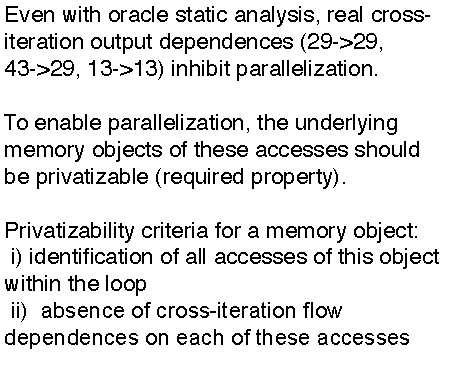
\includegraphics[scale=0.7]{figures/seq_motivation.pdf}
    \end{minipage}

\end{tabular}

\label{fig:dijkstra_motivation}
\caption{Sequential \textit{dijkstra} example from MiBench~\cite{}}
%(with dynamic allocation of arrays (static privatization is not applicable anymore). assume that pathcost cannot be proven as non-liveout)
\end{figure*}


\begin{figure*}
\centering
\begin{tabular}{c|c|c}

  \hspace{1cm}  &  \hspace{0.7cm}  State-of-the-art spec-DOALL system (Privateer)
  \hspace{0.7cm} &  \hspace{3cm} This Work \hspace{3cm}

  \\
  \hline
  \raisebox{2.8cm}[0pt][0pt]{\rotatebox{90}{Compilation Workflow}}
  %\raisebox{1cm}[0pt][0pt]{\rotatebox{90}{\parbox{4cm}{Data Level \\ (Logging &
%Copy-out Cost)}}}
  &
  %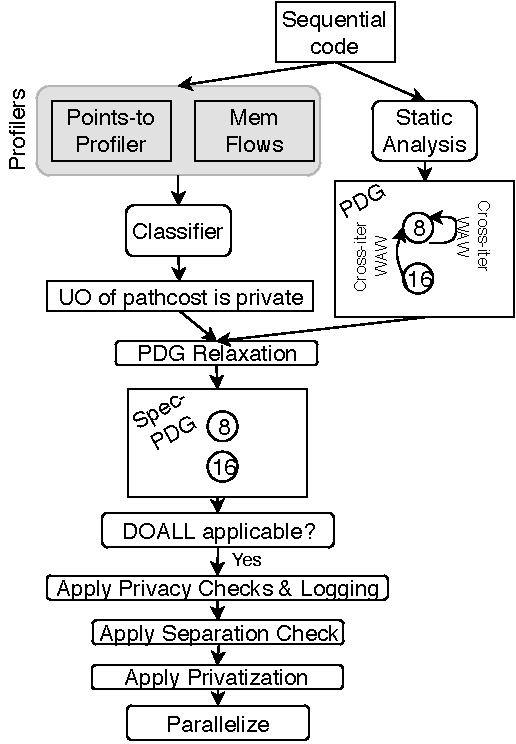
\includegraphics[width=6cm]{figures/compilation_flow_privateer}
  %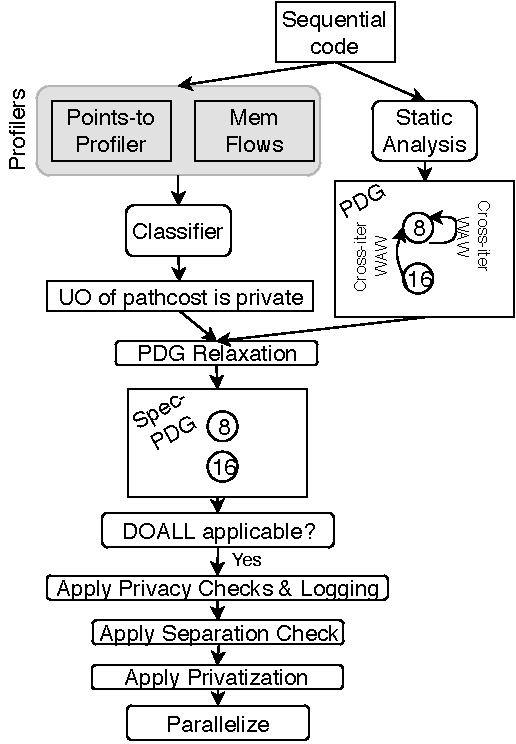
\includegraphics[scale=0.5]{figures/compilation_flow_privateer}
  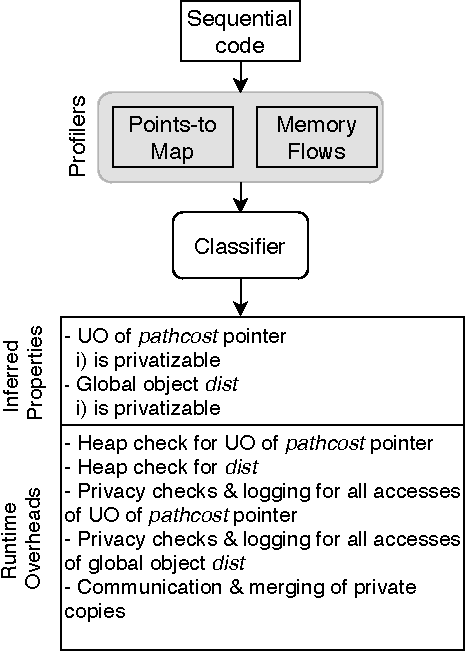
\includegraphics[scale=0.5]{figures/compilation_flow_privateer_ver2}
  &
  %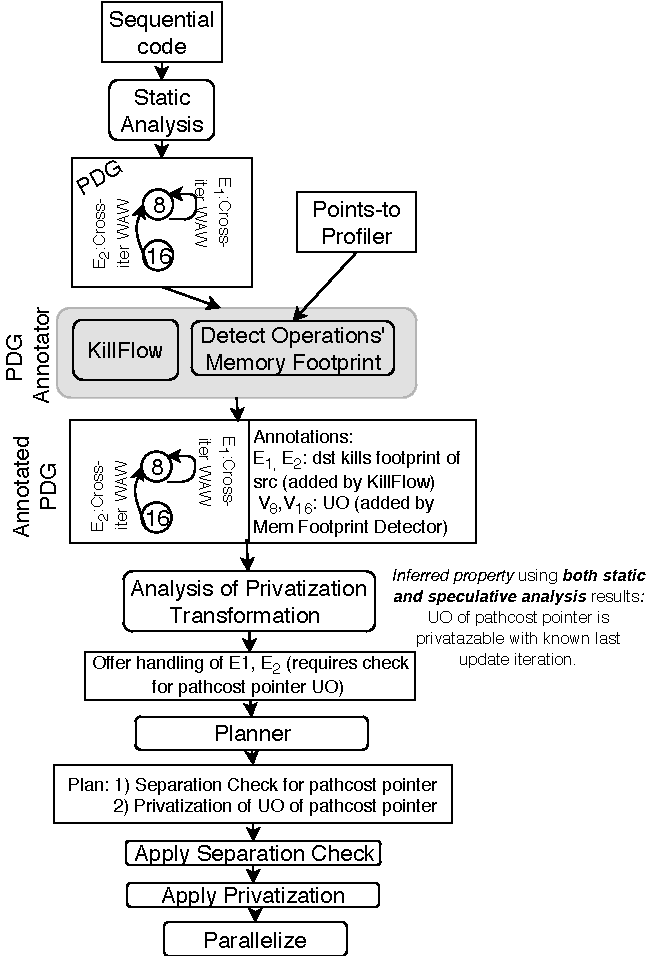
\includegraphics[width=6cm]{figures/compilation_flow_lsd}
  %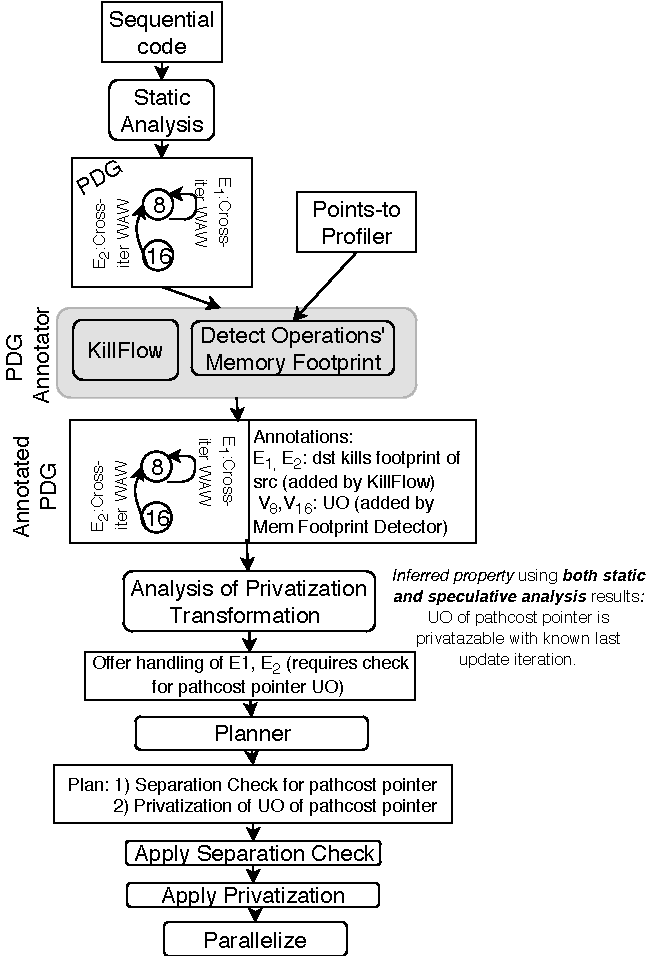
\includegraphics[scale=0.5]{figures/compilation_flow_lsd}
  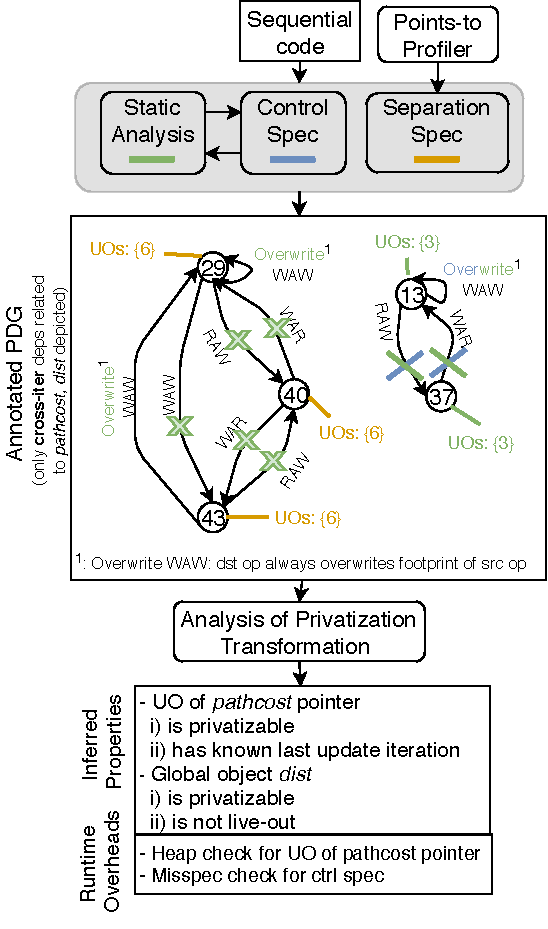
\includegraphics[scale=0.5]{figures/compilation_flow_lsd_ver2}

  \\
  \hline
  \rotatebox[origin=c]{90}{Source Code}
  &
  \scriptsize
  %\tiny
  \subfloat {
  \begin{minipage}{6.6cm}
  \begin{lstlisting}[morekeywords={pathcost}, belowskip=0pt, firstnumber=1,
name=dij_checks]
int *pathcost; // dyn alloc 1-D N
int *adj; // dyn alloc 2-D NxN
int dist, v, src, i;

for (src=0; src<N; src++) {
\end{lstlisting}

\begin{lstlisting}[morekeywords={pathcost}, aboveskip=0pt,belowskip=0pt,backgroundcolor=\color{lightgray},
firstnumber=auto, name=dij_checks]
  // Privacy Check
  private_write(pathcost, N*sizeof(int));
\end{lstlisting}

\begin{lstlisting}[morekeywords={pathcost},aboveskip=0pt, belowskip=0pt, firstnumber=auto,name=dij_checks]
  for (i=0; i<N; i++)
    pathcost[i] = inf;

  enqueue(src, 0);
  while (!emptyQ()) {
    dequeue(&v, &dist);
    for (i=0; i<N; i++) {
      nDist = adj[v][i] + dist;
\end{lstlisting}

\begin{lstlisting}[morekeywords={pathcost}, aboveskip=0pt,belowskip=0pt,backgroundcolor=\color{lightgray},
firstnumber=auto, name=dij_checks]
      // Privacy Check
      private_read(pathcost, sizeof(int));
\end{lstlisting}


\begin{lstlisting}[morekeywords={pathcost}, aboveskip=0pt, belowskip=0pt, firstnumber=auto,name=dij_checks]
      if (pathcost[i] > nDist) {
\end{lstlisting}

\begin{lstlisting}[morekeywords={pathcost}, aboveskip=0pt,belowskip=0pt,backgroundcolor=\color{lightgray},
firstnumber=auto, name=dij_checks]
        // Privacy Check
        private_write(pathcost, sizeof(int));
\end{lstlisting}

\begin{lstlisting}[morekeywords={pathcost}, aboveskip=0pt, belowskip=0pt, firstnumber=auto,name=dij_checks]
        pathcost[i] = nDist;
        enqueue(i, nDist);
      }
    }
  }
}
\end{lstlisting}

  \end{minipage}
  }
  &
  \scriptsize
  %\tiny
  \subfloat {
  \begin{minipage}{6cm}
  %\begin{lstlisting}[morekeywords={pathcost}, belowskip=0pt, firstnumber=1,
%name=dij_checks]
%int *pathcost; // dyn alloc 1-D N
%int *adj; // dyn alloc 2-D NxN
%int dist, v, src, i;


\begin{lstlisting}[morekeywords={pathcost,dist}, belowskip=0pt,
firstnumber=10, name=dij_checks, showlines=true]
int dequeue() {
  if (!emptyQ()) {


\end{lstlisting}

\begin{lstlisting}[morekeywords={pathcost,dist}, aboveskip=0pt, belowskip=0pt,
firstnumber=13, name=dij_checks]
    dist = ...
    ...
  }
\end{lstlisting}

  \begin{lstlisting}[morekeywords={pathcost}, aboveskip=0pt,belowskip=0pt,backgroundcolor=\color{lightgray}, firstnumber=auto, name=dij_checks]
  else // 0% added overhead
    misspec("Control misspec in dequeue()");
\end{lstlisting}

\begin{lstlisting}[morekeywords={pathcost,dist}, aboveskip=0pt, belowskip=0pt,
firstnumber=auto, name=dij_checks,showlines=true]
}

void worker_loop(int start, int N, int step) {

\end{lstlisting}

  \begin{lstlisting}[morekeywords={pathcost}, aboveskip=0pt,belowskip=0pt,backgroundcolor=\color{lightgray},
  firstnumber=auto, name=dij_checks,showlines=true]
  // Separation Local Check -- < 0.001% added overhead
  check_heap(pathcost, OVERWRITE_PRIVATE);
  \end{lstlisting}

\begin{lstlisting}[morekeywords={pathcost}, aboveskip=0pt,
belowskip=0pt, firstnumber=24,name=dij_checks,showlines=true]

  for (src=start; src<N; src+=step) {


\end{lstlisting}
\begin{lstlisting}[morekeywords={pathcost,dist}, aboveskip=0pt,
belowskip=0pt, firstnumber=28,name=dij_checks,showlines=true]
    for (i=0; i<N; i++)
      pathcost[i] = inf;

    enqueue(src, 0);
    while (!emptyQ()) {
      int v = dequeue();
      for (i=0; i<N; i++) {
\end{lstlisting}
\begin{lstlisting}[morekeywords={pathcost,dist,nDist}, aboveskip=0pt,
belowskip=0pt, firstnumber=auto,name=dij_checks,showlines=true]



        nDist = adj[v][i] + dist;
\end{lstlisting}
\begin{lstlisting}[morekeywords={pathcost}, aboveskip=0pt,
belowskip=0pt, firstnumber=auto,name=dij_checks,showlines=true]


        if (pathcost[i] > nDist) {


\end{lstlisting}
\begin{lstlisting}[morekeywords={pathcost}, aboveskip=0pt,
belowskip=0pt, firstnumber=auto,name=dij_checks]
          pathcost[i] = nDist;
          enqueue(i, nDist);
        }
      }
    }
\end{lstlisting}

\begin{lstlisting}[morekeywords={pathcost,dist}, aboveskip=0pt,
belowskip=0pt, firstnumber=auto,name=dij_checks,showlines=true]
  }
\end{lstlisting}

\begin{lstlisting}[morekeywords={pathcost},
aboveskip=0pt,belowskip=0pt,backgroundcolor=\color{lightgray},
firstnumber=auto, name=dij_checks,showlines=true]
  // only last iter's pathcost array
  // needs to be communicated -- < 1% added overhead
  if (src == N-1+step)
    communicate_pathcost();
\end{lstlisting}

\begin{lstlisting}[morekeywords={pathcost}, aboveskip=0pt,
belowskip=0pt, firstnumber=auto,name=dij_checks]
}
\end{lstlisting}

  \end{minipage}
  }

  \\
  \hline
  \raisebox{1cm}[0pt][0pt]{\rotatebox{90}{Data Flow}}
  %\raisebox{1cm}[0pt][0pt]{\rotatebox{90}{\parbox{4cm}{Data Level \\ (Logging &
%Copy-out Cost)}}}
  &
  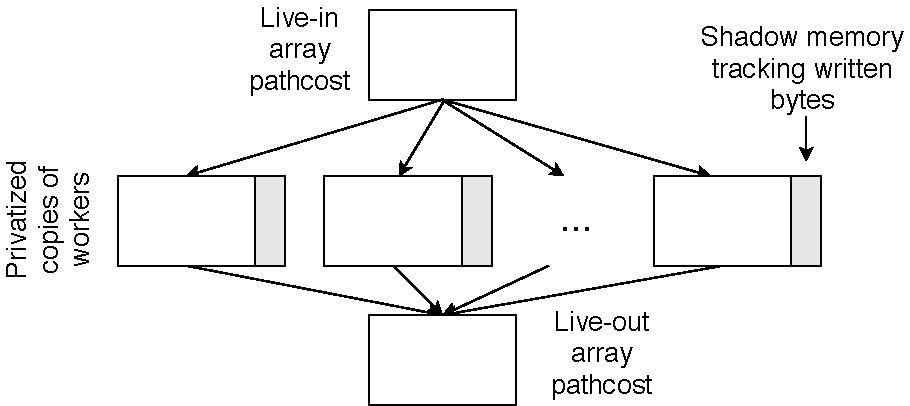
\includegraphics[width=6.5cm]{figures/data_view_privateer}
  &
  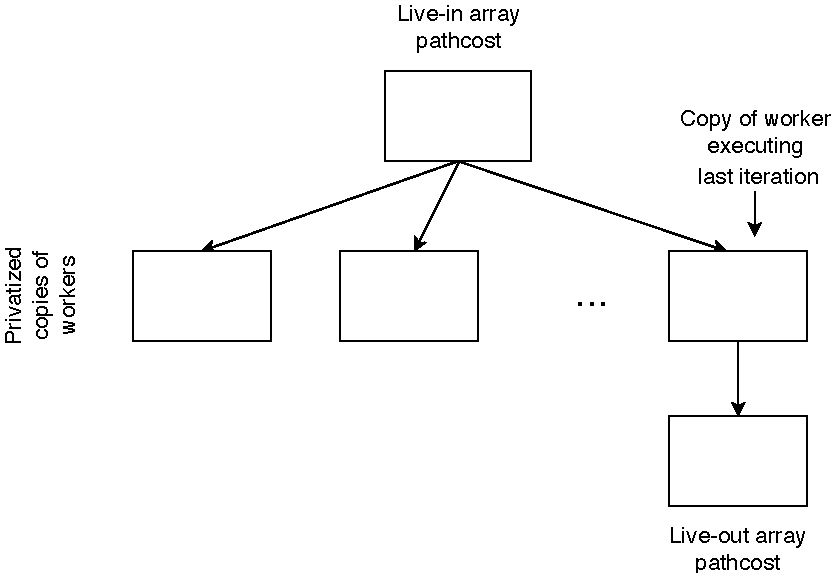
\includegraphics[width=6cm]{figures/data_view_lsd}

\end{tabular}

\caption{Parallelization of hot loop of \textit{dijkstra} benchmark}
\label{fig:dijkstra_parallelized}
\end{figure*}

%\begin{figure*}[t]
%  \centering
%  \scriptsize
%  \subfloat[Sequential dijkstra example]
%  {
%    \label{fig:dijkstra_motivation}
%    \begin{minipage}{4.4cm}
%      \begin{lstlisting}[morekeywords={pathcost,dist}, aboveskip=0pt, belowskip=0pt, firstnumber=1]
int *pathcost; // dyn alloc 1-D N
int *adj; // dyn alloc 2-D NxN
int dist;
int nDist;

void allocatePathCost() {
  pathcost = (int*)malloc(N*sizeof(int));
}

int dequeue() {
  if (!emptyQ()) {
\end{lstlisting}

\begin{lstlisting}[morekeywords={pathcost,dist}, aboveskip=0pt, belowskip=0pt,
firstnumber=13, name=dij_checks]
    dist = ...
    ...
  }
\end{lstlisting}

\begin{lstlisting}[morekeywords={pathcost,dist}, aboveskip=0pt, belowskip=0pt,
firstnumber=18, name=dij_checks]
}

void hot_loop(int N) {
\end{lstlisting}
\begin{lstlisting}[morekeywords={pathcost}, aboveskip=0pt, belowskip=0pt,
firstnumber=25]
  for (src=0; src<N; src++) {
\end{lstlisting}
\begin{lstlisting}[morekeywords={pathcost,dist}, aboveskip=0pt, belowskip=0pt,
firstnumber=28]
    for (i=0; i<N; i++)
      pathcost[i] = inf;

    enqueue(src, 0);
    while (!emptyQ()) {
      int v = dequeue();
      for (i=0; i<N; i++) {
\end{lstlisting}
\begin{lstlisting}[morekeywords={pathcost,dist}, aboveskip=0pt,
belowskip=0pt, firstnumber=38,name=dij_checks]
        nDist = adj[v][i] + dist;
\end{lstlisting}
\begin{lstlisting}[morekeywords={pathcost}, aboveskip=0pt, belowskip=0pt,
firstnumber=41]
        if (pathcost[i] > nDist) {
\end{lstlisting}
\begin{lstlisting}[morekeywords={pathcost}, aboveskip=0pt, belowskip=0pt,
firstnumber=44]
          pathcost[i] = nDist;
          enqueue(i, nDist);
        }
      }
    }
\end{lstlisting}
\begin{lstlisting}[morekeywords={pathcost}, aboveskip=0pt,
belowskip=0pt, firstnumber=52]
  }
\end{lstlisting}
\begin{lstlisting}[morekeywords={pathcost}, aboveskip=0pt,
belowskip=0pt, firstnumber=54]
}
\end{lstlisting}

%    \end{minipage}
%  }
%  \hspace{0.3cm}
%  \subfloat[Parallelized code with state-of-the-art spec-DOALL system (Privateer)]
%  {
%    \label{fig:dijkstra_motivation_checks}
%    \begin{minipage}{6.6cm}
%      \begin{lstlisting}[morekeywords={pathcost}, belowskip=0pt, firstnumber=1,
name=dij_checks]
int *pathcost; // dyn alloc 1-D N
int *adj; // dyn alloc 2-D NxN
int dist, v, src, i;

for (src=0; src<N; src++) {
\end{lstlisting}

\begin{lstlisting}[morekeywords={pathcost}, aboveskip=0pt,belowskip=0pt,backgroundcolor=\color{lightgray},
firstnumber=auto, name=dij_checks]
  // Privacy Check
  private_write(pathcost, N*sizeof(int));
\end{lstlisting}

\begin{lstlisting}[morekeywords={pathcost},aboveskip=0pt, belowskip=0pt, firstnumber=auto,name=dij_checks]
  for (i=0; i<N; i++)
    pathcost[i] = inf;

  enqueue(src, 0);
  while (!emptyQ()) {
    dequeue(&v, &dist);
    for (i=0; i<N; i++) {
      nDist = adj[v][i] + dist;
\end{lstlisting}

\begin{lstlisting}[morekeywords={pathcost}, aboveskip=0pt,belowskip=0pt,backgroundcolor=\color{lightgray},
firstnumber=auto, name=dij_checks]
      // Privacy Check
      private_read(pathcost, sizeof(int));
\end{lstlisting}


\begin{lstlisting}[morekeywords={pathcost}, aboveskip=0pt, belowskip=0pt, firstnumber=auto,name=dij_checks]
      if (pathcost[i] > nDist) {
\end{lstlisting}

\begin{lstlisting}[morekeywords={pathcost}, aboveskip=0pt,belowskip=0pt,backgroundcolor=\color{lightgray},
firstnumber=auto, name=dij_checks]
        // Privacy Check
        private_write(pathcost, sizeof(int));
\end{lstlisting}

\begin{lstlisting}[morekeywords={pathcost}, aboveskip=0pt, belowskip=0pt, firstnumber=auto,name=dij_checks]
        pathcost[i] = nDist;
        enqueue(i, nDist);
      }
    }
  }
}
\end{lstlisting}

%    \end{minipage}
%  }
%  \hspace{0.3cm}
%  \subfloat[Parallelized code with minimal overhead (this work)]
%  {
%    \label{fig:dijkstra_motivation_checks}
%    \begin{minipage}{5.4cm}
%      %\begin{lstlisting}[morekeywords={pathcost}, belowskip=0pt, firstnumber=1,
%name=dij_checks]
%int *pathcost; // dyn alloc 1-D N
%int *adj; // dyn alloc 2-D NxN
%int dist, v, src, i;


\begin{lstlisting}[morekeywords={pathcost,dist}, belowskip=0pt,
firstnumber=10, name=dij_checks, showlines=true]
int dequeue() {
  if (!emptyQ()) {


\end{lstlisting}

\begin{lstlisting}[morekeywords={pathcost,dist}, aboveskip=0pt, belowskip=0pt,
firstnumber=13, name=dij_checks]
    dist = ...
    ...
  }
\end{lstlisting}

  \begin{lstlisting}[morekeywords={pathcost}, aboveskip=0pt,belowskip=0pt,backgroundcolor=\color{lightgray}, firstnumber=auto, name=dij_checks]
  else // 0% added overhead
    misspec("Control misspec in dequeue()");
\end{lstlisting}

\begin{lstlisting}[morekeywords={pathcost,dist}, aboveskip=0pt, belowskip=0pt,
firstnumber=auto, name=dij_checks,showlines=true]
}

void worker_loop(int start, int N, int step) {

\end{lstlisting}

  \begin{lstlisting}[morekeywords={pathcost}, aboveskip=0pt,belowskip=0pt,backgroundcolor=\color{lightgray},
  firstnumber=auto, name=dij_checks,showlines=true]
  // Separation Local Check -- < 0.001% added overhead
  check_heap(pathcost, OVERWRITE_PRIVATE);
  \end{lstlisting}

\begin{lstlisting}[morekeywords={pathcost}, aboveskip=0pt,
belowskip=0pt, firstnumber=24,name=dij_checks,showlines=true]

  for (src=start; src<N; src+=step) {


\end{lstlisting}
\begin{lstlisting}[morekeywords={pathcost,dist}, aboveskip=0pt,
belowskip=0pt, firstnumber=28,name=dij_checks,showlines=true]
    for (i=0; i<N; i++)
      pathcost[i] = inf;

    enqueue(src, 0);
    while (!emptyQ()) {
      int v = dequeue();
      for (i=0; i<N; i++) {
\end{lstlisting}
\begin{lstlisting}[morekeywords={pathcost,dist,nDist}, aboveskip=0pt,
belowskip=0pt, firstnumber=auto,name=dij_checks,showlines=true]



        nDist = adj[v][i] + dist;
\end{lstlisting}
\begin{lstlisting}[morekeywords={pathcost}, aboveskip=0pt,
belowskip=0pt, firstnumber=auto,name=dij_checks,showlines=true]


        if (pathcost[i] > nDist) {


\end{lstlisting}
\begin{lstlisting}[morekeywords={pathcost}, aboveskip=0pt,
belowskip=0pt, firstnumber=auto,name=dij_checks]
          pathcost[i] = nDist;
          enqueue(i, nDist);
        }
      }
    }
\end{lstlisting}

\begin{lstlisting}[morekeywords={pathcost,dist}, aboveskip=0pt,
belowskip=0pt, firstnumber=auto,name=dij_checks,showlines=true]
  }
\end{lstlisting}

\begin{lstlisting}[morekeywords={pathcost},
aboveskip=0pt,belowskip=0pt,backgroundcolor=\color{lightgray},
firstnumber=auto, name=dij_checks,showlines=true]
  // only last iter's pathcost array
  // needs to be communicated -- < 1% added overhead
  if (src == N-1+step)
    communicate_pathcost();
\end{lstlisting}

\begin{lstlisting}[morekeywords={pathcost}, aboveskip=0pt,
belowskip=0pt, firstnumber=auto,name=dij_checks]
}
\end{lstlisting}

%    \end{minipage}
%  }
%
%  \caption{Sequential \textit{dijkstra} code and parallelized versions. Function
%worker\_loop is executed by each worker after spawning. Function's inputs
%specify which iterations each worker should run. Checks, logging and copy-out
%operations are in grey. Assume that array \textit{pathcost} cannot be proved as
%non-liveout.}
%
%\end{figure*}


%\lstset{basicstyle=\ttfamily, numbers=left, numberstyle=\tiny,
%  stepnumber=1, numbersep=5pt}
%\begin{figure*}[t]
%  \centering
%  \scriptsize
%  \subfloat[Privateer]
%  {
%    \label{fig:data_view_privateer}
%    \begin{minipage}{7cm}
%      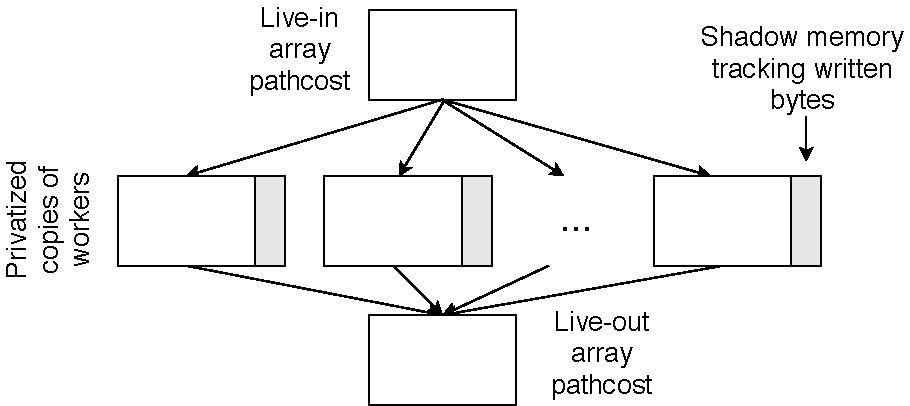
\includegraphics[width=\textwidth]{figures/data_view_privateer}
%    \end{minipage}
%  }
%  \hspace{2cm}
%  \subfloat[This work]
%  {
%    \label{fig:data_view_lsd}
%    \begin{minipage}{7cm}
%      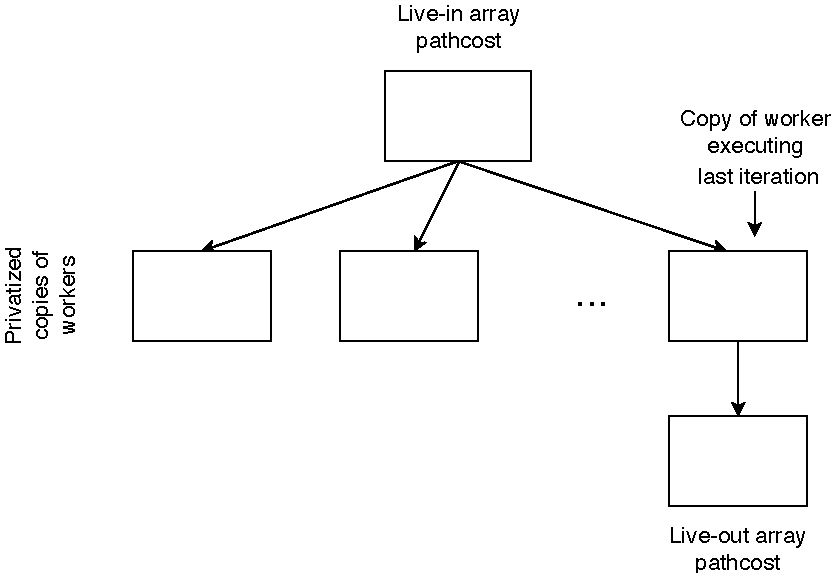
\includegraphics[width=\textwidth]{figures/data_view_lsd}
%    \end{minipage}
%  }
%  \caption{Data view}
%
%\end{figure*}


%
%%showcases how fine-grained collaboration between static analysis and speculative
%%assumptions can infer high-level program properties without the need for
%%expensive memory speculation.
%
%%Dependence has three conditions. We say there is a memorydependence  from
%%instructioni1to  instructioni2iff(alias)the footprint of operationi1may-aliasthe
%%footprint ofi2, and(feasible-path) there is a feasible path of execution
%%fromi1toi2which (no-kill) does not contain an operation which over-writes the
%%common memory footprint. Footprint denotes theset of memory locations read or
%%written by the instruction.
%
%1) global object \textit{g\_qCount}
%
%\textbf{Static analysis and inexpensive speculation in isolation}:
%%
%%Analysis Results:
%Static analysis cannot disprove all loop-carried RAW and WAW dependences on
%accesses of g\_qCount.
%%
%Profile information indicates that the first load of g\_qCount in each iteration
%always returns zero.  Using this information, value prediction removes the
%loop-carried RAW dependence sinking on this load.
%%
%Removal of this dependence prevents usage of memory speculation for this
%particular load.
%%
%Presence of WAW dependences though necessitates privatization of the memory
%object, and value prediction cannot reason about store instructions and cannot
%give any additional information related to output dependences.
%%
%%Cost
%The cost in this case includes the validation overhead for value prediction
%(perform load before loop exits or on backedges and compared predicted value
%with loaded value) and the privatizaition cost (monitor stores participating in
%the WAW dependences to determine last written value). Bookkeping for
%privatization is the dominant cost as it requires updating metadata multiple
%times per loop iteration (given that some stores are within inner loops).
%%dynamic resolution to determine last written value
%
%
%\textbf{Collaboration of static and speculative analysis}:
%%
%This value prediction can be seen as a store before the first load of g\_qCount
%that kills any data flow for this memory object from previous iterations.
%%
%An extended speculative analysis removes, similarly to the first case, the
%loop-carried RAW dependence, but additionally queries alias analysis for
%must-aliasing accesses with the load's address. If these accesses are dominated
%by the load, then loop-carried RAW or WAW dependences from or to these accesses
%can be ignored.
%%
%This remvoes the need to perform dynamic resolution of the last written value;
%the final content of this memory location is predictable.
%%any action to log (for last write) any of these individual memory operations.
%%
%%Interestingly, this case of privatization goes beyond the classical definition
%%of privatization definition~\cite{tu-padua-array-privatization-1994}  that
%%requires that every load of a privatizable element is preceded by a store to
%%the element in the same iteration of the loop. In this scenario, global
%%variable g\_qCount is first loaded at every iteration, a data flow exists.
%%
%%
%The cost in this case only includes the small validation overhead for value
%prediction. There is no bookkeping cost for privatization.
%%
%No prior work could detect and so effectively handle this new case of
%privatization.
%%- privatization cost: none avoid dynamic resolution to determine last written
%%value (live-out value)
%
%%TODO: use this first
%2) global object \textit{iPrev}
%
%- speculative assumption: the branch "if (qHead)" is always taken (control speculation)
%
%- static analysis: alias analysis, killflow, noCaptureGlobal analysis passes
%
%- validation cost: no validation cost for control spec (just misspecs if branch
%  is not taken)
%
%- Using the speculative assumption, killflow analysis can infer that the store
%  in line 15 kills all other accesses of this global
%variable (killed operations are identified by quering alias analysis). Given this
%property, any RAW loop-carried dependence is disproved.  Additionally, static
%analysis can enumerate all uses of this global, since it is not captured, and
%detect that this global is used only within this loop, namely it is not a
%live-out.  Thus, there is no need to log stores and keep track of the last
%written value to it.
%
%%3) TODO: example with blackscholes
%
%For all the above memory objects, Privateer~\cite{}, the state-of-the-art DOALL
%system that we mainly compare against, would require expensive logging on most
%of their accesses,
%%either for validation checks or for identifying who wrote last what
%yielding sub-optimal speedups as clearly exhibited by our experimental results
%in section ~\ref{eval}.
%%all these objects are classified as privatizable by Privateer
%
%Note that our framework is not limited to static global allocations.  It can
%handle linked or recursive data structures, pointers,type  casts,  and  dynamic
%allocation.
%
%%use alvinn for value pred + alias analysis
%
%%Note that WAR dependences can be ignored thanks to the process-based runtime
%%system.



This work is motivated by this excessive use of memory speculation and expensive
privatization of prior speculative systems that significantly limits their
efficiency.
%
We show that use of cheap-to-validatate speculation in conjuction with static
analysis allows inferance of high-level properties that prevent expensive
bookkeeping and checks.
